
%% bare_jrnl.tex
%% V1.4a
%% 2014/09/17
%% by Michael Shell
%% see http://www.michaelshell.org/
%% for current contact information.
%%
%% This is a skeleton file demonstrating the use of IEEEtran.cls
%% (requires IEEEtran.cls version 1.8a or later) with an IEEE
%% journal paper.
%%
%% Support sites:
%% http://www.michaelshell.org/tex/ieeetran/
%% http://www.ctan.org/tex-archive/macros/latex/contrib/IEEEtran/
%% and
%% http://www.ieee.org/

%%*************************************************************************
%% Legal Notice:
%% This code is offered as-is without any warranty either expressed or
%% implied; without even the implied warranty of MERCHANTABILITY or
%% FITNESS FOR A PARTICULAR PURPOSE! 
%% User assumes all risk.
%% In no event shall IEEE or any contributor to this code be liable for
%% any damages or losses, including, but not limited to, incidental,
%% consequential, or any other damages, resulting from the use or misuse
%% of any information contained here.
%%
%% All comments are the opinions of their respective authors and are not
%% necessarily endorsed by the IEEE.
%%
%% This work is distributed under the LaTeX Project Public License (LPPL)
%% ( http://www.latex-project.org/ ) version 1.3, and may be freely used,
%% distributed and modified. A copy of the LPPL, version 1.3, is included
%% in the base LaTeX documentation of all distributions of LaTeX released
%% 2003/12/01 or later.
%% Retain all contribution notices and credits.
%% ** Modified files should be clearly indicated as such, including  **
%% ** renaming them and changing author support contact information. **
%%
%% File list of work: IEEEtran.cls, IEEEtran_HOWTO.pdf, bare_adv.tex,
%%                    bare_conf.tex, bare_jrnl.tex, bare_conf_compsoc.tex,
%%                    bare_jrnl_compsoc.tex, bare_jrnl_transmag.tex
%%*************************************************************************


% *** Authors should verify (and, if needed, correct) their LaTeX system  ***
% *** with the testflow diagnostic prior to trusting their LaTeX platform ***
% *** with production work. IEEE's font choices and paper sizes can       ***
% *** trigger bugs that do not appear when using other class files.       ***                          ***
% The testflow support page is at:
% http://www.michaelshell.org/tex/testflow/



\documentclass[journal]{IEEEtran}
%
% If IEEEtran.cls has not been installed into the LaTeX system files,
% manually specify the path to it like:
% \documentclass[journal]{../sty/IEEEtran}


\usepackage{amsmath,graphicx}
\usepackage{amsfonts}
\usepackage{bm}
\usepackage{amsthm}
\newtheorem{proposition}{Proposition}



% Some very useful LaTeX packages include:
% (uncomment the ones you want to load)


% *** MISC UTILITY PACKAGES ***
%
%\usepackage{ifpdf}
% Heiko Oberdiek's ifpdf.sty is very useful if you need conditional
% compilation based on whether the output is pdf or dvi.
% usage:
% \ifpdf
%   % pdf code
% \else
%   % dvi code
% \fi
% The latest version of ifpdf.sty can be obtained from:
% http://www.ctan.org/tex-archive/macros/latex/contrib/oberdiek/
% Also, note that IEEEtran.cls V1.7 and later provides a builtin
% \ifCLASSINFOpdf conditional that works the same way.
% When switching from latex to pdflatex and vice-versa, the compiler may
% have to be run twice to clear warning/error messages.






% *** CITATION PACKAGES ***
%
%\usepackage{cite}
% cite.sty was written by Donald Arseneau
% V1.6 and later of IEEEtran pre-defines the format of the cite.sty package
% \cite{} output to follow that of IEEE. Loading the cite package will
% result in citation numbers being automatically sorted and properly
% "compressed/ranged". e.g., [1], [9], [2], [7], [5], [6] without using
% cite.sty will become [1], [2], [5]--[7], [9] using cite.sty. cite.sty's
% \cite will automatically add leading space, if needed. Use cite.sty's
% noadjust option (cite.sty V3.8 and later) if you want to turn this off
% such as if a citation ever needs to be enclosed in parenthesis.
% cite.sty is already installed on most LaTeX systems. Be sure and use
% version 5.0 (2009-03-20) and later if using hyperref.sty.
% The latest version can be obtained at:
% http://www.ctan.org/tex-archive/macros/latex/contrib/cite/
% The documentation is contained in the cite.sty file itself.






% *** GRAPHICS RELATED PACKAGES ***
%
\ifCLASSINFOpdf
  % \usepackage[pdftex]{graphicx}
  % declare the path(s) where your graphic files are
  % \graphicspath{{../pdf/}{../jpeg/}}
  % and their extensions so you won't have to specify these with
  % every instance of \includegraphics
  % \DeclareGraphicsExtensions{.pdf,.jpeg,.png}
\else
  % or other class option (dvipsone, dvipdf, if not using dvips). graphicx
  % will default to the driver specified in the system graphics.cfg if no
  % driver is specified.
  % \usepackage[dvips]{graphicx}
  % declare the path(s) where your graphic files are
  % \graphicspath{{../eps/}}
  % and their extensions so you won't have to specify these with
  % every instance of \includegraphics
  % \DeclareGraphicsExtensions{.eps}
\fi
% graphicx was written by David Carlisle and Sebastian Rahtz. It is
% required if you want graphics, photos, etc. graphicx.sty is already
% installed on most LaTeX systems. The latest version and documentation
% can be obtained at: 
% http://www.ctan.org/tex-archive/macros/latex/required/graphics/
% Another good source of documentation is "Using Imported Graphics in
% LaTeX2e" by Keith Reckdahl which can be found at:
% http://www.ctan.org/tex-archive/info/epslatex/
%
% latex, and pdflatex in dvi mode, support graphics in encapsulated
% postscript (.eps) format. pdflatex in pdf mode supports graphics
% in .pdf, .jpeg, .png and .mps (metapost) formats. Users should ensure
% that all non-photo figures use a vector format (.eps, .pdf, .mps) and
% not a bitmapped formats (.jpeg, .png). IEEE frowns on bitmapped formats
% which can result in "jaggedy"/blurry rendering of lines and letters as
% well as large increases in file sizes.
%
% You can find documentation about the pdfTeX application at:
% http://www.tug.org/applications/pdftex





% *** MATH PACKAGES ***
%
%\usepackage[cmex10]{amsmath}
% A popular package from the American Mathematical Society that provides
% many useful and powerful commands for dealing with mathematics. If using
% it, be sure to load this package with the cmex10 option to ensure that
% only type 1 fonts will utilized at all point sizes. Without this option,
% it is possible that some math symbols, particularly those within
% footnotes, will be rendered in bitmap form which will result in a
% document that can not be IEEE Xplore compliant!
%
% Also, note that the amsmath package sets \interdisplaylinepenalty to 10000
% thus preventing page breaks from occurring within multiline equations. Use:
%\interdisplaylinepenalty=2500
% after loading amsmath to restore such page breaks as IEEEtran.cls normally
% does. amsmath.sty is already installed on most LaTeX systems. The latest
% version and documentation can be obtained at:
% http://www.ctan.org/tex-archive/macros/latex/required/amslatex/math/





% *** SPECIALIZED LIST PACKAGES ***
%
%\usepackage{algorithmic}
% algorithmic.sty was written by Peter Williams and Rogerio Brito.
% This package provides an algorithmic environment fo describing algorithms.
% You can use the algorithmic environment in-text or within a figure
% environment to provide for a floating algorithm. Do NOT use the algorithm
% floating environment provided by algorithm.sty (by the same authors) or
% algorithm2e.sty (by Christophe Fiorio) as IEEE does not use dedicated
% algorithm float types and packages that provide these will not provide
% correct IEEE style captions. The latest version and documentation of
% algorithmic.sty can be obtained at:
% http://www.ctan.org/tex-archive/macros/latex/contrib/algorithms/
% There is also a support site at:
% http://algorithms.berlios.de/index.html
% Also of interest may be the (relatively newer and more customizable)
% algorithmicx.sty package by Szasz Janos:
% http://www.ctan.org/tex-archive/macros/latex/contrib/algorithmicx/




% *** ALIGNMENT PACKAGES ***
%
%\usepackage{array}
% Frank Mittelbach's and David Carlisle's array.sty patches and improves
% the standard LaTeX2e array and tabular environments to provide better
% appearance and additional user controls. As the default LaTeX2e table
% generation code is lacking to the point of almost being broken with
% respect to the quality of the end results, all users are strongly
% advised to use an enhanced (at the very least that provided by array.sty)
% set of table tools. array.sty is already installed on most systems. The
% latest version and documentation can be obtained at:
% http://www.ctan.org/tex-archive/macros/latex/required/tools/


% IEEEtran contains the IEEEeqnarray family of commands that can be used to
% generate multiline equations as well as matrices, tables, etc., of high
% quality.




% *** SUBFIGURE PACKAGES ***
%\ifCLASSOPTIONcompsoc
%  \usepackage[caption=false,font=normalsize,labelfont=sf,textfont=sf]{subfig}
%\else
%  \usepackage[caption=false,font=footnotesize]{subfig}
%\fi
% subfig.sty, written by Steven Douglas Cochran, is the modern replacement
% for subfigure.sty, the latter of which is no longer maintained and is
% incompatible with some LaTeX packages including fixltx2e. However,
% subfig.sty requires and automatically loads Axel Sommerfeldt's caption.sty
% which will override IEEEtran.cls' handling of captions and this will result
% in non-IEEE style figure/table captions. To prevent this problem, be sure
% and invoke subfig.sty's "caption=false" package option (available since
% subfig.sty version 1.3, 2005/06/28) as this is will preserve IEEEtran.cls
% handling of captions.
% Note that the Computer Society format requires a larger sans serif font
% than the serif footnote size font used in traditional IEEE formatting
% and thus the need to invoke different subfig.sty package options depending
% on whether compsoc mode has been enabled.
%
% The latest version and documentation of subfig.sty can be obtained at:
% http://www.ctan.org/tex-archive/macros/latex/contrib/subfig/




% *** FLOAT PACKAGES ***
%
%\usepackage{fixltx2e}
% fixltx2e, the successor to the earlier fix2col.sty, was written by
% Frank Mittelbach and David Carlisle. This package corrects a few problems
% in the LaTeX2e kernel, the most notable of which is that in current
% LaTeX2e releases, the ordering of single and double column floats is not
% guaranteed to be preserved. Thus, an unpatched LaTeX2e can allow a
% single column figure to be placed prior to an earlier double column
% figure. The latest version and documentation can be found at:
% http://www.ctan.org/tex-archive/macros/latex/base/


%\usepackage{stfloats}
% stfloats.sty was written by Sigitas Tolusis. This package gives LaTeX2e
% the ability to do double column floats at the bottom of the page as well
% as the top. (e.g., "\begin{figure*}[!b]" is not normally possible in
% LaTeX2e). It also provides a command:
%\fnbelowfloat
% to enable the placement of footnotes below bottom floats (the standard
% LaTeX2e kernel puts them above bottom floats). This is an invasive package
% which rewrites many portions of the LaTeX2e float routines. It may not work
% with other packages that modify the LaTeX2e float routines. The latest
% version and documentation can be obtained at:
% http://www.ctan.org/tex-archive/macros/latex/contrib/sttools/
% Do not use the stfloats baselinefloat ability as IEEE does not allow
% \baselineskip to stretch. Authors submitting work to the IEEE should note
% that IEEE rarely uses double column equations and that authors should try
% to avoid such use. Do not be tempted to use the cuted.sty or midfloat.sty
% packages (also by Sigitas Tolusis) as IEEE does not format its papers in
% such ways.
% Do not attempt to use stfloats with fixltx2e as they are incompatible.
% Instead, use Morten Hogholm'a dblfloatfix which combines the features
% of both fixltx2e and stfloats:
%
% \usepackage{dblfloatfix}
% The latest version can be found at:
% http://www.ctan.org/tex-archive/macros/latex/contrib/dblfloatfix/




%\ifCLASSOPTIONcaptionsoff
%  \usepackage[nomarkers]{endfloat}
% \let\MYoriglatexcaption\caption
% \renewcommand{\caption}[2][\relax]{\MYoriglatexcaption[#2]{#2}}
%\fi
% endfloat.sty was written by James Darrell McCauley, Jeff Goldberg and 
% Axel Sommerfeldt. This package may be useful when used in conjunction with 
% IEEEtran.cls'  captionsoff option. Some IEEE journals/societies require that
% submissions have lists of figures/tables at the end of the paper and that
% figures/tables without any captions are placed on a page by themselves at
% the end of the document. If needed, the draftcls IEEEtran class option or
% \CLASSINPUTbaselinestretch interface can be used to increase the line
% spacing as well. Be sure and use the nomarkers option of endfloat to
% prevent endfloat from "marking" where the figures would have been placed
% in the text. The two hack lines of code above are a slight modification of
% that suggested by in the endfloat docs (section 8.4.1) to ensure that
% the full captions always appear in the list of figures/tables - even if
% the user used the short optional argument of \caption[]{}.
% IEEE papers do not typically make use of \caption[]'s optional argument,
% so this should not be an issue. A similar trick can be used to disable
% captions of packages such as subfig.sty that lack options to turn off
% the subcaptions:
% For subfig.sty:
% \let\MYorigsubfloat\subfloat
% \renewcommand{\subfloat}[2][\relax]{\MYorigsubfloat[]{#2}}
% However, the above trick will not work if both optional arguments of
% the \subfloat command are used. Furthermore, there needs to be a
% description of each subfigure *somewhere* and endfloat does not add
% subfigure captions to its list of figures. Thus, the best approach is to
% avoid the use of subfigure captions (many IEEE journals avoid them anyway)
% and instead reference/explain all the subfigures within the main caption.
% The latest version of endfloat.sty and its documentation can obtained at:
% http://www.ctan.org/tex-archive/macros/latex/contrib/endfloat/
%
% The IEEEtran \ifCLASSOPTIONcaptionsoff conditional can also be used
% later in the document, say, to conditionally put the References on a 
% page by themselves.




% *** PDF, URL AND HYPERLINK PACKAGES ***
%
%\usepackage{url}
% url.sty was written by Donald Arseneau. It provides better support for
% handling and breaking URLs. url.sty is already installed on most LaTeX
% systems. The latest version and documentation can be obtained at:
% http://www.ctan.org/tex-archive/macros/latex/contrib/url/
% Basically, \url{my_url_here}.




% *** Do not adjust lengths that control margins, column widths, etc. ***
% *** Do not use packages that alter fonts (such as pslatex).         ***
% There should be no need to do such things with IEEEtran.cls V1.6 and later.
% (Unless specifically asked to do so by the journal or conference you plan
% to submit to, of course. )


% correct bad hyphenation here
\hyphenation{}


\begin{document}
%
% paper title
% Titles are generally capitalized except for words such as a, an, and, as,
% at, but, by, for, in, nor, of, on, or, the, to and up, which are usually
% not capitalized unless they are the first or last word of the title.
% Linebreaks \\ can be used within to get better formatting as desired.
% Do not put math or special symbols in the title.
\title{Modulation Design for MIMO-CoMP HARQ}
%
%
% author names and IEEE memberships
% note positions of commas and nonbreaking spaces ( ~ ) LaTeX will not break
% a structure at a ~ so this keeps an author's name from being broken across
% two lines.
% use \thanks{} to gain access to the first footnote area
% a separate \thanks must be used for each paragraph as LaTeX2e's \thanks
% was not built to handle multiple paragraphs
%

\author{
  Wenhao Wu,~\IEEEmembership{Student Member,~IEEE,}
  Hans Mittelmann,
  Zhi Ding,~\IEEEmembership{Fellow,~IEEE}
  \thanks{
    This work was supported in part by the National Science Foundation
    under Grants CNS-1443870, ECCS-1307820, and CCF-1321143. The work of the
    second author was supported in part by AFOSR under grant FA 9550-15-1-0351.
  }% <-this % stops a space
}

% note the % following the last \IEEEmembership and also \thanks - 
% these prevent an unwanted space from occurring between the last author name
% and the end of the author line. i.e., if you had this:
% 
% \author{....lastname \thanks{...} \thanks{...} }
%                     ^------------^------------^----Do not want these spaces!
%
% a space would be appended to the last name and could cause every name on that
% line to be shifted left slightly. This is one of those "LaTeX things". For
% instance, "\textbf{A} \textbf{B}" will typeset as "A B" not "AB". To get
% "AB" then you have to do: "\textbf{A}\textbf{B}"
% \thanks is no different in this regard, so shield the last } of each \thanks
% that ends a line with a % and do not let a space in before the next \thanks.
% Spaces after \IEEEmembership other than the last one are OK (and needed) as
% you are supposed to have spaces between the names. For what it is worth,
% this is a minor point as most people would not even notice if the said evil
% space somehow managed to creep in.



% The paper headers
%\markboth{Journal of \LaTeX\ Class Files,~Vol.~13, No.~9, September~2014}%
%{Shell \MakeLowercase{\textit{et al.}}: Bare Demo of IEEEtran.cls for Journals}
% The only time the second header will appear is for the odd numbered pages
% after the title page when using the twoside option.
% 
% *** Note that you probably will NOT want to include the author's ***
% *** name in the headers of peer review papers.                   ***
% You can use \ifCLASSOPTIONpeerreview for conditional compilation here if
% you desire.




% If you want to put a publisher's ID mark on the page you can do it like
% this:
%\IEEEpubid{0000--0000/00\$00.00~\copyright~2014 IEEE}
% Remember, if you use this you must call \IEEEpubidadjcol in the second
% column for its text to clear the IEEEpubid mark.



% use for special paper notices
%\IEEEspecialpapernotice{(Invited Paper)}




% make the title area
\maketitle

% As a general rule, do not put math, special symbols or citations
% in the abstract or keywords.
\begin{abstract}
  %\boldmath
  % (what we do)
  Modulation diversity (MoDiv) is a simple and practical transmission
  enhancement technique that utilizes different modulation mappings to reduce
  packet loss rate and achieve higher link throughput. MoDiv is particularly
  meaningful and effective in hybrid-ARQ (HARQ) systems. We study the deployment
  and optimization of MoDiv for HARQ in a MIMO-coordinated multi-point
  (MIMO-CoMP) scenario under Rician fading channel to mitigate packet loss.
    % (how they do)
    % (how we do)
  We formulate the design optimization of MoDiv into a quadratic
  three-dimensional assignment problem (Q3AP), then solve it using a modified
  iterated local search (ILS) method. Numerical results demonstrate clear
  performance gain over simple retransmissions and over a heuristic design
  under fading channels.
  
\end{abstract}

% Note that keywords are not normally used for peerreview papers.
\begin{IEEEkeywords}
  MoDiv, MIMO, CoMP, HARQ, Q3AP.
\end{IEEEkeywords}






% For peer review papers, you can put extra information on the cover
% page as needed:
% \ifCLASSOPTIONpeerreview
% \begin{center} \bfseries EDICS Category: 3-BBND \end{center}
% \fi
%
% For peerreview papers, this IEEEtran command inserts a page break and
% creates the second title. It will be ignored for other modes.
\IEEEpeerreviewmaketitle

\section{Introduction}
\label{sec:intro}

In wireless data communication systems, high rate transmission under poor
channel conditions often leads to reception errors. To recover lost packets,
Automatic Repeat reQuest (ARQ) or Hybrid ARQ (HARQ) are important mechanisms for
improving reliability at both network layer~\cite{TS36.331} and PHY
layer~\cite{TS36.213}. Constellation Rearrangement (CoRe) is a pragmatic
technique that provides additional robustness via Modulation Diversity (MoDiv)
to HARQ system~\cite{benelli1992new}.
As linear modulations of $Q$-ary constellations such as PSK, QAM are usually
adopted in practical wireless communications systems, the same string of
$\log_2Q$ bits can be mapped to different symbols across the multiple HARQ
(re)transmissions. This technique has been studied for point-to-point
HARQ~\cite{samra2005symbol}, relay
networks~\cite{seddik2008trans, khormuji2008rate} and
relay-HARQ~\cite{kim2009design, ryu2011ber, wu2016modulation} and is shown to
greatly improve the BER performance and throughput.

Also, in recent years, coordinated multipoint (CoMP) transmission has become a
promising technique which has been supported by
LTE-Advanced~\cite{sawahashi2010coordinated}. By coordinating multiple base
stations/remote radio heads (RRHs) from different cells/sectors, CoMP can
effectively improve cell edge user data rate and spectral
efficiency~\cite{irmer2011coordinated}. When applied to CoMP, MoDiv faces great
opportunities and challenges at the same time which has not been fully understood. On the one hand,
it is possible to adopt different constellation remapping schemes at different
transmitters, which could potentially provide larger diversity gain. On the
other hand, the optimization of more than one constellation mapping for each
round of retransmission is non-trivial, especially when perfect channel state
information (CSI) is not available.
In this work, we propose a MoDiv design scheme for a CoMP system composed of one
user equipment (UE) and two cooperative transmitters connected to a centralized
control unit. We assume independent Rician fading MIMO channel between the transmitters
and the UE, which is more general and practical than existing works on
MIMO-CoRe~\cite{bahadori2014performance, zhao2009harq}.
The CoRe is designed to minimize the expected bit error rate (BER) under
statistical CSI assumption after each (re)transmission. The resulting
optimization problem has a Successive Quadratic 3 Dimensional Assignment Problem
(Q3AP) formulation~\cite{hahn2008quadratic}. Although Q3AP is generally NP-hard and
cannot be solved exactly except for trivially small constellations, an
efficient modified Iterated Local Search (ILS) approach is adopted. Our
numerical results demonstrate significant gains achieved by the MoDiv techniques
in various simulation settings and performance measurements.


% Structure of the manuscript
%The paper is organized as follows. Section~\ref{sec:model} introduces the
%TWRC-AF model and the HARQ protocol we are using. Section~\ref{sec:modiv}
%presents the successive BER minimization MoDiv design problem. In
%Section~\ref{sec:numerical}, we present the numerical results to show the
%performance gain of our MoDiv scheme. Finally, Section~\ref{sec:conclusion}
%concludes the paper.


% needed in second column of first page if using \IEEEpubid
%\IEEEpubidadjcol

\section{System Model}
\label{sec:model}
% MoDiv as an enhancement of beamforming, 
Consider the constellation rearrangement (CoRe) in a HARQ-enabled MIMO-CoMP
downlink channel composed of two transmitters and one UE. For the original
transmission, bits are mapped to constellation symbols using conventional Gray mapping for both transmitters. However, in order to
maximize the signal space diversity as an enhancement of beamforming, we allow
different mappings of the same sequence of information bits at the two
transmitters during the HARQ process. We assume a HARQ protocol based on Chase
Combining (CC) and a maximum number of $M$ retransmissions.
For the $m$-th (re)transmission, $m=0,1,\ldots,M$ where $m=0$ represents the
original transmission, every consecutive $\log_2Q$ bits are encoded into a label
$p=0,\ldots, Q-1$ and then mapped to two constellation symbols via a vector
mapping function $\bm{\psi}^{(m)}[p] = [\psi_1^{(m)}[p], \psi_2^{(m)}[p]]^T$,
where $\psi_a^{(m)}[p]\in \mathcal{C}$ and $\mathcal{C}$ is the set of
constellation symbols (e.g. QAM, 16-QAM). The two symbols are then transmitted
at the two transmitters, respectively. The received signal at the $m$-th
(re)transmission of the bit sequence corresponding to label $p$ is:
\begin{align}
  \mathbf{y}^{(m)} & =  \mathbf{A}^{(m)}\bm{\psi}^{(m)}[p] + \mathbf{n}^{(m)}
  \notag \\
  & =\mathbf{H}_1^{(m)}\mathbf{p}_1 \psi_1^{(m)}[p] +
  \mathbf{H}_2^{(m)}\mathbf{p}_2 \psi_2^{(m)}[p] + \mathbf{n}^{(m)},
\end{align}
where $\mathbf{H}_a^{(m)}$ is a $N_R$-by-$N_{T,a}$ MIMO channel between the
$a$-th transmitter and the UE, $\mathbf{p}_a$ is a $N_{T,a}$-by-1 linear beamformer
for the $a$-th transmitter, $a=1, 2$, and the additive noise
$\mathbf{n}^{(m)}\sim\mathcal{CN}(\mathbf{0}, \sigma^2\mathbf{I})$. We
assume the elements of $\mathbf{H}_a^{(m)}$ follow correlated Rician
distributed channel~\cite{taricco2007optimum} independent across retransmissions
and between the two transmitters.
Specifically,
\begin{align}
    \mathbf{H}_a^{(m)} = \sqrt{\frac{K_a}{K_a+1}}\bar{\mathbf{H}}_{a} +
    \sqrt{\frac{1}{K_a+1}}
    \mathbf{R}^{1/2}\mathbf{H}_{w,a}^{(m)}\mathbf{T}_a^{1/2},\; 
\end{align}
for $a=1,2$ where the $N_R$-by-$N_R$ matrix $\mathbf{R}$ and the $N_{T,
a}$-by-$N_{T,a}$ matrix $\mathbf{T}_a$ are the receive and transmit covariance matrices,
respectively, while $\bar{\mathbf{H}}_{a}$ represents the line-of-sight
component and $\mathbf{H}_{w,a}^{(m)}$ is a random matrix composed of
independent entries of $\mathcal{CN}(0,1)$. Here we denote $\mathbf{A}^{(m)} =
[\mathbf{H}_1^{(m)}\mathbf{p}_1, \mathbf{H}_2^{(m)}\mathbf{p}_2]$ as the
equivalent MIMO channel from the two transmitters to the UE during the $m$-th
retransmission.

After the $m$-th retransmission, the receiver attempts to
demodulate $p$ by combining all the symbols received so far with the ML
detection:
\begin{align}
    p^* = \arg\min_p\sum_{n = 0}^{m}\left\|\mathbf{y}^{(n)} -
    \sum_{a=1,2}\mathbf{H}_a^{(n)}\mathbf{p}_a\psi_a^{(n)}[p]\right\|^2.
\end{align}

\section{Successive Constellation Mapping Design For Modulation Diversity}
\label{sec:modiv}
% Outline

\subsection{A BER Upper Bound}
\label{ssec:ber}
The BER of the ML demodulator after the $m$-th (re)transmission can be
upper-bounded and approximated by
\begin{align}
  P_{BER}^{(m)} = \sum_{p=0}^{Q - 1}\sum_{q=0}^{Q - 1}\frac{B[p,
  q]}{Q}P_{PEP}^{(m)}(q|p) \label{eq:P_BER}
\end{align}
where $B[p, q]$ is the Hamming distance between the binary
representation of $p$ and $q$ divided by $\log_2Q$ as
in~\cite{samra2005symbol}. The computation of $P_{PEP}(q|p)$, the pairwise
error probability (PEP) of mistakenly decoding $p$ into $q$, generally follows
the procedure in~\cite{han2009performance}:
\begin{align}
    P_{PEP}^{(m)}(q|p) & = \mathbb{E}
    \left[Q\left(\sqrt{\sum_{n=0}^m\frac{\|\mathbf{A}^{(n)}
    \mathbf{e}^{(n)}[p,q]\|^2} {2\sigma^2}}\right)\right]
    \label{eq:PEP_M}
\end{align}
where $\mathbf{e}^{(n)}[p,q] = [e_1^{(n)}[p,q], e_2^{(n)}[p,q]]^T =
\bm{\psi}^{(n)}[p] - \bm{\psi}^{(n)}[q]$.
Since the $Q$-function can be bounded as $Q(x)\leq e^{-x^2/2}/2$~\cite{proakisdigital},
the PEP in~(\ref{eq:PEP_M}) can be upper bounded by
\begin{align}
    \tilde{P}_{PEP}^{(m)}(q|p) & =
    \frac{1}{2} \prod_{n=0}^{m}
    \mathbb{E}\left[\exp\left(-\frac{\|\mathbf{A}^{(n)}
    \mathbf{e}^{(n)}[p,q]\|^2}{4\sigma^2}\right)\right]
    \label{eq:PEP_M_1}
\end{align}
Denote $E_n[p,q]$ as the expectation in Eq.~(\ref{eq:PEP_M_1}), which
facilitates the recursion $\tilde{P}_{PEP}^{(m)}(q|p) =
\tilde{P}_{PEP}^{(m-1)}(q|p)E_m[p,q]$, $\tilde{P}_{PEP}^{(-1)}(q|p)=1/2$.
$E_n[p,q]$ can be evaluated as follows:
\begin{proposition}
  \begin{align}
    E_n[p,q] & =
    \frac{(4\sigma^2)^{N_R}\exp\left(-\bm{\mu}_n^H[p,q]\mathbf{S}_n^{-1}[p,q]\bm{\mu}_n[p,q]\right)}
    {\det(\mathbf{S}_n[p,q])} \label{eq:E}\\
     \mathbf{S}_n[p,q] & =
    4\sigma^2\mathbf{I} +
    \sum_{a=1,2} \frac{|e_a^{(n)}[p,q]|^2 \mathbf{p}_a^H\mathbf{T}_a
    \mathbf{p}_a}{K_a+1} \mathbf{R},\notag\\
    \bm{\mu}_n[p,q] & = \sum_{a=1,2}
    \sqrt{\frac{K_a}{K_a+1}}\bar{\mathbf{H}}_a\mathbf{p}_ae_a^{(n)}[p,q].
    \label{eq:S_mu}
  \end{align}
  \label{prop:en}
\end{proposition}
\begin{proof}
  We have $\mathbf{A}^{(n)}\mathbf{e}_n[p,q]
  \sim\mathcal{CN}(\bm{\mu}_n[p,q], \mathbf{C}_n[p,q])$
  where 
  \begin{align}
    \mathbf{C}_n[p,q] = \sum_{a=1,2}
    \frac{|e_a^{(n)}[p,q]|^2\mathbf{p}_a^H\mathbf{T}_a
    \mathbf{p}_a}{K_a+1}\mathbf{R}.
  \end{align}
  For $\mathbf{v}\sim\mathcal{CN}(\bm{\mu}, \mathbf{C})$, using the technique of
  completing the square~\cite[Sec. 2.3.1]{bishop2006pattern}, it is easy to show
  \begin{align}
    \mathbb{E}\left[\exp(-\lambda\|\mathbf{v}\|^2)\right] =
    \frac{\exp\left(-\bm{\mu}^H(\lambda^{-1}\mathbf{I} +
    \mathbf{C})^{-1}\bm{\mu}\right)}{\det(\mathbf{I} +
    \lambda\mathbf{C})} \label{eq:elv2}
  \end{align}
  which in turn leads to Proposition~\ref{prop:en}.
\end{proof}

\subsection{Successive Quadratic 3-D Assignment Problem (S-Q3AP)}
\label{ssec:q3ap}
Our MoDiv design aims to solve
\begin{align}
  \min_{\bm{\psi}^{(m)}|\bm{\psi}^{(n)},
  n=0,\ldots,m-1}\tilde{P}_{BER}^{(m)},m=1,\ldots,M,\label{eq:minber}
\end{align}
where $\tilde{P}_{BER}^{(m)}$ is the approximated version of
$P_{BER}^{(m)}$ by substituting $P_{PEP}^{(m)}(q|p)$ with
$\tilde{P}_{PEP}^{(m)}(q|p)$. Denote the 3-D permutation matrix
$\mathbf{x}^{(m)} = \{x_{pij}^{(m)}|p,i,j=0,\ldots,Q-1\}$ as an equivalent
representation of $\bm{\psi}^{(m)}$ by $x_{pij}^{(m)} =
\delta(\bm{\psi}^{(m)}[p], [\psi_0[i], \psi_0[j]]^T)$ and $\delta(x,y)$ is the
Kronecker delta function, $\psi_0$ represents Gray mapping, which must satisfy
\begin{align}
  \mathcal{S} & = \left\{\mathbf{x}:\,\sum_{p=0}^{Q-1}x_{pij}=
  \sum_{i=0}^{Q-1}x_{pij} =\sum_{j=0}^{Q-1}x_{pij} =1\right\}.
  \label{eq:constraint}
\end{align}
Then Eq.~(\ref{eq:minber}) can be formulated into a S-Q3AP as follows:
\begin{align}
  \min_{\mathbf{x}^{(m)}\in \mathcal{S}}
  \sum_{p=0}^{Q-1}\sum_{i=0}^{Q-1}\sum_{j=0}^{Q-1}
  \sum_{q=0}^{Q-1}\sum_{k=0}^{Q-1}\sum_{l=0}^{Q-1}
  f_{pq}^{(m)}d_{ikjl}x_{pij}^{(m)}x_{qkl}^{(m)},
  \label{eq:SQ3AP}
\end{align}
where
\begin{subequations}
  \begin{align}
    f_{pq}^{(m)} & = \frac{B[p,q]}{Q}\tilde{P}_{PEP}^{(m-1)}(q|p) \\
    d_{ikjl} & =
    \frac{(4\sigma^2)^{N_R}
    \exp(-\bm{\mu}_{ikjl}^H\mathbf{S}_{ikjl}^{-1}\bm{\mu}_{ikjl})} {\det(\mathbf{S}_{ikjl})}
  \end{align}
\end{subequations}
Here $d_{ikjl}$ is derived from Eq.~\eqref{eq:E}\eqref{eq:S_mu} with
\begin{align}
  \mathbf{S}_{ikjl} & = 4\sigma^2\mathbf{I} + \left(\frac{|e_{ik}|^2
  \mathbf{p}_1^H\mathbf{T}_1 \mathbf{p}_1}{K_1+1} + \frac{|e_{jl}|^2
  \mathbf{p}_2^H\mathbf{T}_2 \mathbf{p}_2}{K_2+1}\right) \mathbf{R},\notag\\
  \bm{\mu}_{ikjl} & = \sqrt{\frac{K_1}{K_1+1}}\bar{\mathbf{H}}_1\mathbf{p}_1
  e_{ik} + \sqrt{\frac{K_2}{K_2+1}}\bar{\mathbf{H}}_2\mathbf{p}_2e_{jl}.
\end{align}
and $e_{ik} = \psi_0[i] - \psi_0[k]$, $e_{jl} = \psi_0[j] - \psi_0[l]$.
$f_{pq}^{(m)}$ can be updated recursively while solving the S-Q3AP, since:
\begin{align}
  \tilde{P}_{PEP}^{(m)}(q|p) & =
  \sum_{i,k,j,l=0}^{Q-1}\tilde{P}_{PEP}^{(m-1)}(q|p)d_{ikjl}
  \hat{x}_{pij}^{(m)}\hat{x}_{qkl}^{(m)}
  \label{eq:pep_update}
\end{align}
and $ \tilde{P}_{PEP}^{(-1)}(q|p) = 1/2$. Due to the geometry
of the QAM constellation, the evaluation of $d_{ikjl}$ is actually $\mathcal{O}(Q^2)$ instead of $\mathcal{O}(Q^4)$, and
it only needs to be evaluated once. Consequently, the main computational
complexity lies in solving the Q3AP problems instead of evaluating their
coefficients.

For typical constellations used in modern wireless communication systems such as
16-QAM and 64-QAM, it is impractical to apply the exact branch-and-bound
algorithm~\cite{hahn2008quadratic}. Also, our tests show that they do not have
enough symmetry to exploit for faster solution as does the 16-PSK
constellation~\cite{mittelmann2015solving}.
Consequently, the MoDiv problem is solved with the ILS
method~\cite[Sec. 5.5]{hahn2008quadratic} extended from its QAP
version~\cite{stutzle2006iterated}. The only difference of our
implementation from the one in these references is that, as in
Eq.~(\ref{eq:SQ3AP}) a Q3AP is defined with a 4-D matrix and a 2-D matrix
instead of the general Q3AP defined with a 6-D
matrix~\cite[Eq.(2)]{hahn2008quadratic}. The outline of ILS-Q3AP is as
follows: starting from a random initial mappings $\bm{\psi}=[\psi_1,
\psi_2]$, the algorithm repeatedly executes a local search by exchanging the
mappings of 2 labels whenever the objective function is reduced so as to lower
the objective function and update the mapping locally. When the process hits a
local minimum, it executes a perturbation step to break from it and explore new
solutions by exchanging the mappings of $k_p$ labels, where integer $k_p$ is
adaptively adjusted within a range $[k_{p,min}, k_{p,max}]$. The perturbation is
accepted with a probability defined as in simulated annealing, after which the
local search is restarted from the new mappings until the stopping criterion is
satisfied. The algorithm is meant to be executed in the centralized control
unit connected to the two transmitters.

\section{Numerical Results}
\label{sec:numerical}
Unless otherwise noted, we adopt the following
settings throughout our simulation. For the MIMO-CoMP channel, we have $N_R=1$
and $N_{T, 1} = N_{T, 2} = 2$. The correlation matrices at both transmitters are
$\mathbf{T}_1 = \mathbf{T}_2 =[1,0.7;0,7,1]$, while the line-of-sight (LOS)
components of the Rician channel are set to $\bar{\mathbf{H}}_{1} = [0.2540;
0.2457]$ and $\bar{\mathbf{H}}_{2} = [-0.1027; -0.2320]$, 
The Rician coefficients are $K_1 = K_2 = 4$ by default. A simple maximum SNR
beamformer (MSNRB)~\cite{barriac2006space} (generalized for MIMO channel) under
a total power constraint is used at the two transmitters. 
The maximum number of HARQ retransmissions is set
to $M=4$. Three MoDiv schemes are compared, namely the simple retransmission with
no MoDiv, a heuristic CoRe scheme proposed for
HSDPA~\cite{panasonic2001enhanced} generalized to our CoMP scenario by fixing
$\psi_1 = \psi_2$ and our Q3AP-based MoDiv design, denoted
as NM$m$, CR$m$ and Q3AP$m$, respectively for $m$ retransmissions. The original
transmission using Gray mapping is labeled as TR0. 64-QAM is considered in our
simulations, for which each Q3AP is solved with 5 random initializations and
several minutes of ILS iterations.

First we compare the upper bound and Monte-Carlo average of the uncoded BER for
different $\sigma^2$ in Fig.~\ref{fig:uncoded_noisepower_approx} and 
Fig.~\ref{fig:uncoded_noisepower_mc}.
Apparently, the BER upper bound in~\eqref{eq:P_BER} appears to be a descent
indicator of the actual BER when comparing different MoDiv schemes, and the Q3AP
solution offers a substantial performance gain over the other 2 schemes. For
instance, at low SNR regime Q3AP1 achieves almost the same uncoded BER as NM2,
and Q3AP3 is comparable to CR4.

In Fig.~\ref{fig:uncoded_K_approx} and Fig.~\ref{fig:uncoded_K_mc}, the uncoded
BER is plotted against varying $K$ under fixed $\sigma^2 = 18$dB for $m=1,2$ and 
$\sigma^2 = 8$dB for $m=3,4$. A significant performance gain is observed for all
channel conditions ranging from heavily Rayleigh fading (small $K$) to very
light fading (large $K$).
\begin{figure}[!t]
  \begin{minipage}[b]{.48\linewidth}
    \centering
    \centerline{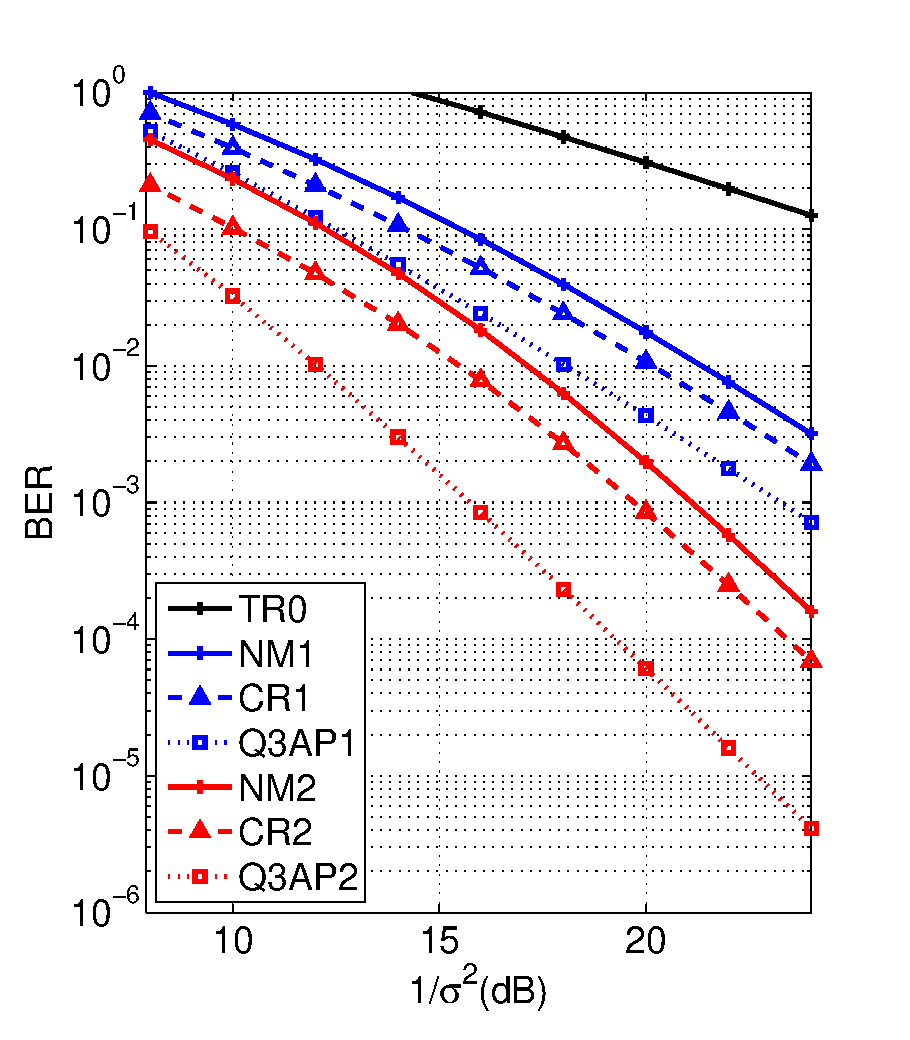
\includegraphics[width=4.5cm]{./figs/BER_noise_power_upperbound_64QAM_12.eps}}
    \centerline{(a) $m=1,2$}\medskip
  \end{minipage}
  \hfill
  \begin{minipage}[b]{0.48\linewidth}
    \centering
    \centerline{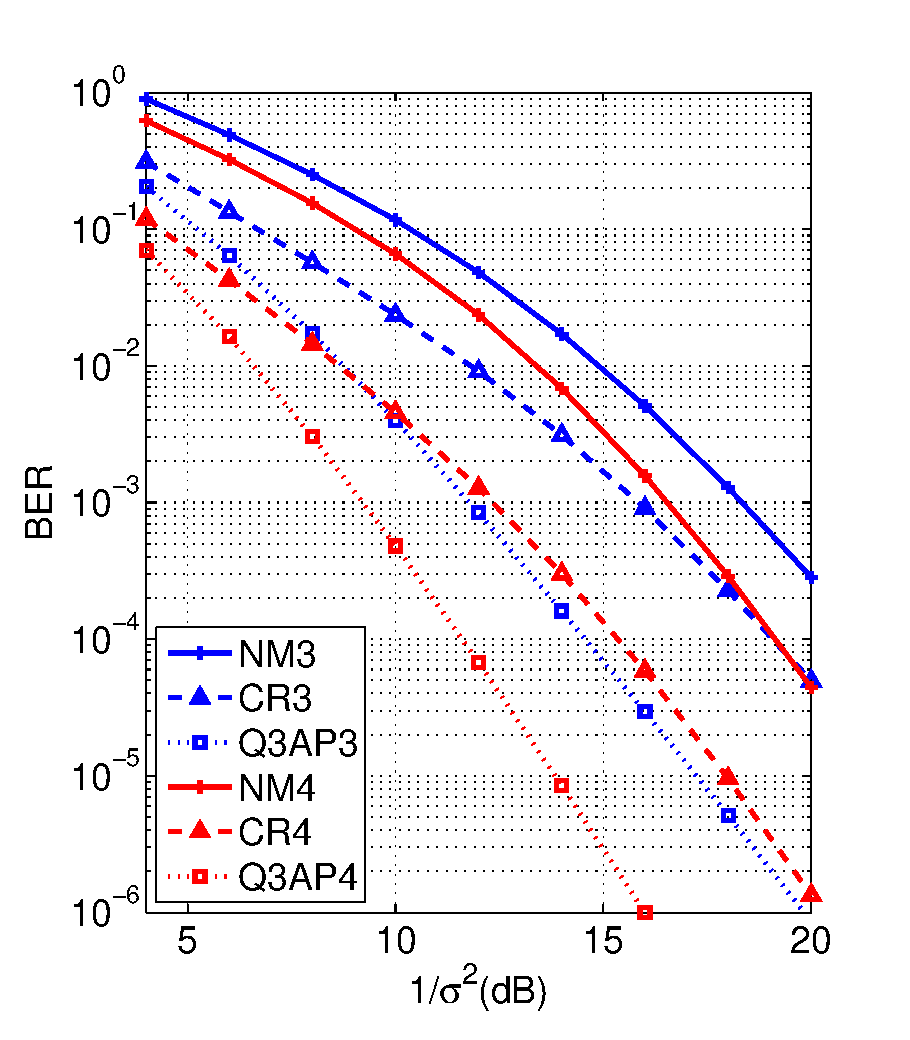
\includegraphics[width=4.5cm]{./figs/BER_noise_power_upperbound_64QAM_34.eps}}
    \centerline{(b) $m=3,4$}\medskip
  \end{minipage}
  \vspace{-10pt}
  \caption{Analytical approximation results of uncoded BER.}
  \label{fig:uncoded_noisepower_approx}
\end{figure}
\begin{figure}[!t]
  \begin{minipage}[b]{.48\linewidth}
    \centering
    \centerline{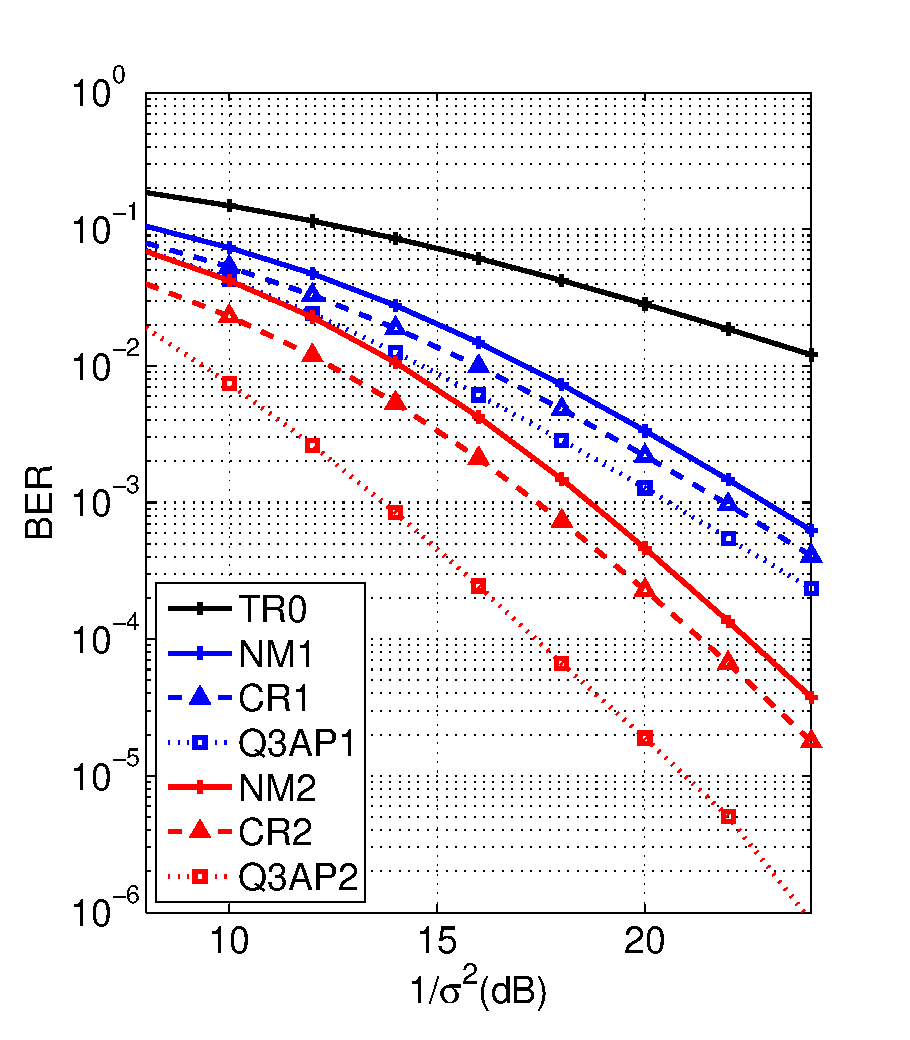
\includegraphics[width=4.5cm]{./figs/BER_noise_power_MonteCarlo_64QAM_12.eps}}
    \centerline{(a) $m=1,2$}\medskip
  \end{minipage}
  \hfill
  \begin{minipage}[b]{0.48\linewidth}
    \centering
    \centerline{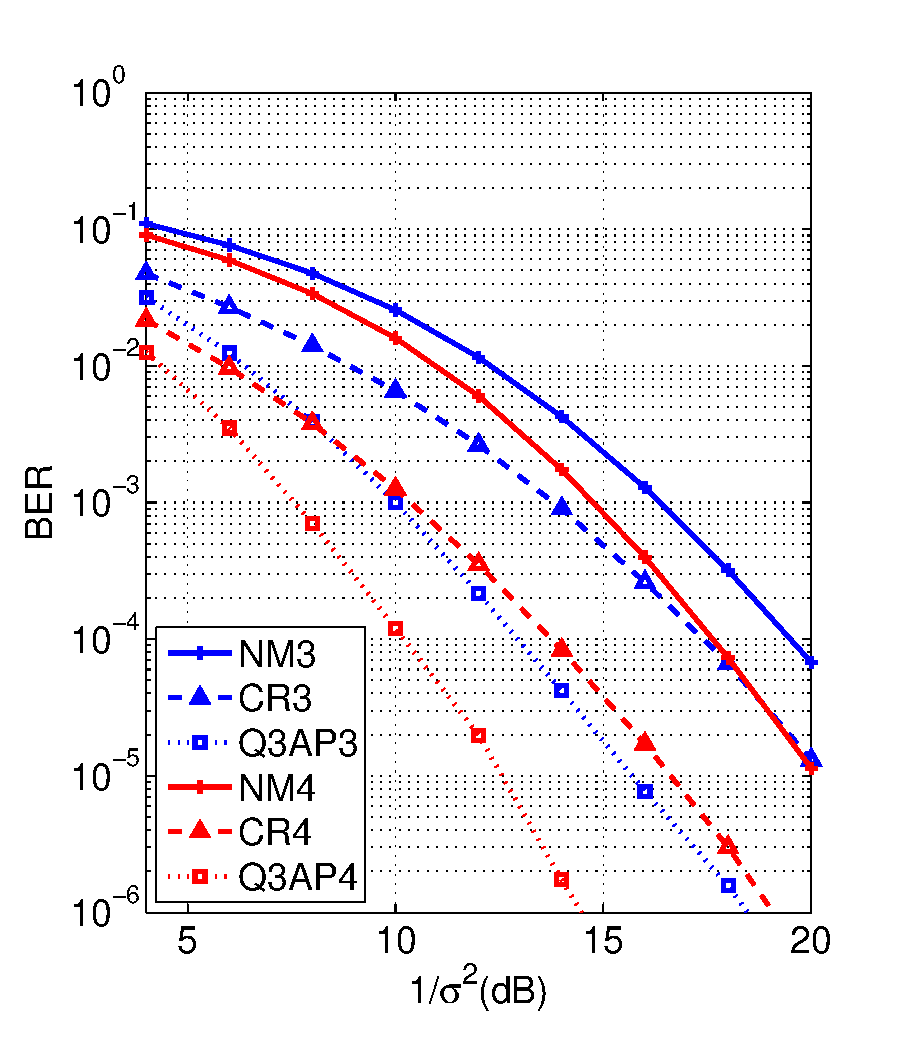
\includegraphics[width=4.5cm]{./figs/BER_noise_power_MonteCarlo_64QAM_34.eps}}
    \centerline{(b) $m=3,4$}\medskip
  \end{minipage}
  \vspace{-10pt}
  \caption{Monte-Carlo simulation results of uncoded BER.}
  \label{fig:uncoded_noisepower_mc}
\end{figure}
\begin{figure}[!t]
  \begin{minipage}[b]{.48\linewidth}
    \centering
    \centerline{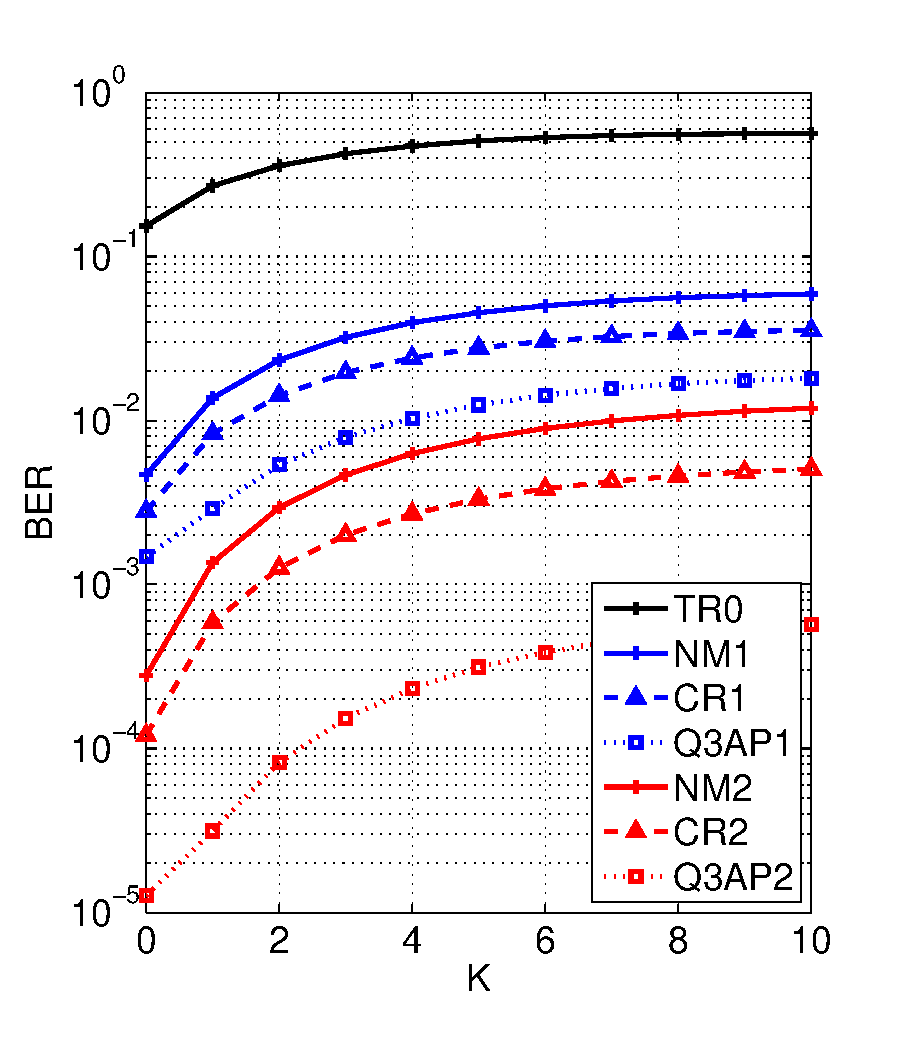
\includegraphics[width=4.5cm]{./figs/BER_K_upperbound_64QAM_12.eps}}
    \centerline{(a) $m=1,2$}\medskip
  \end{minipage}
  \hfill
  \begin{minipage}[b]{0.48\linewidth}
    \centering
    \centerline{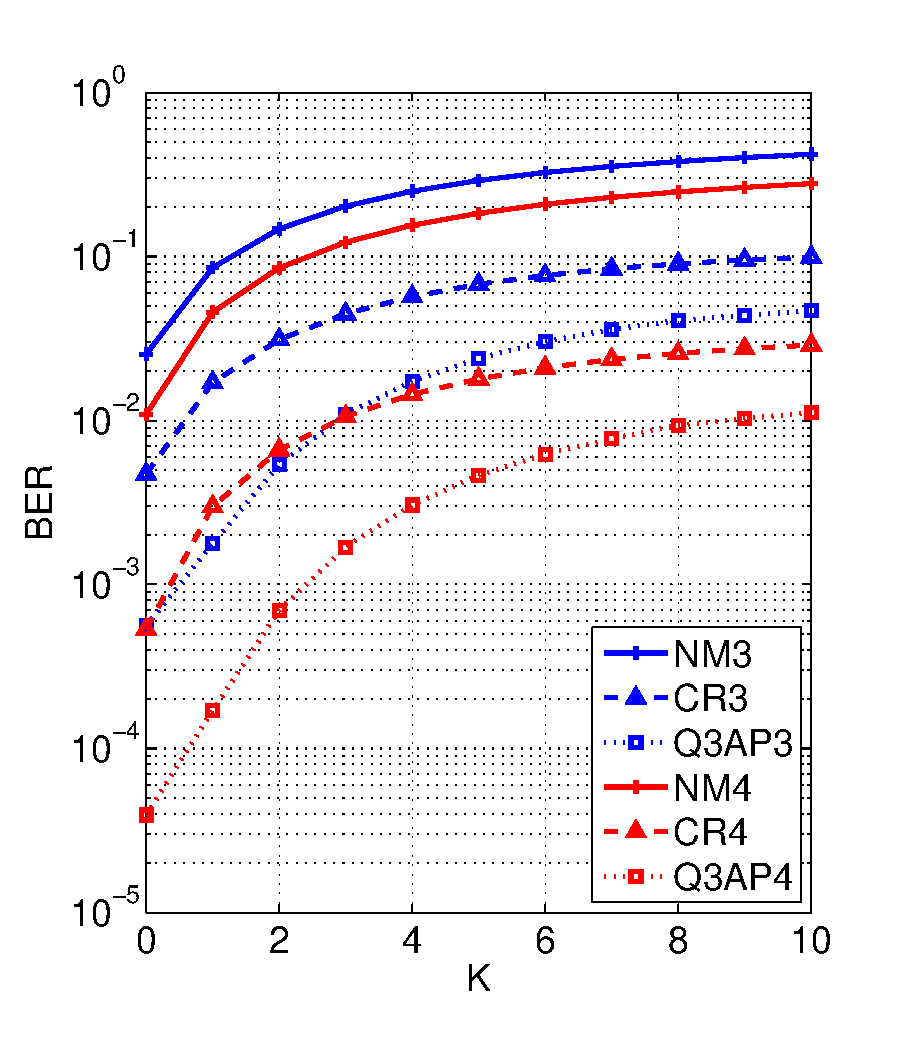
\includegraphics[width=4.5cm]{./figs/BER_K_upperbound_64QAM_34.eps}}
    \centerline{(b) $m=3,4$}\medskip
  \end{minipage}
  \vspace{-10pt}
  \caption{Analytical approximation results of uncoded BER.}
  \label{fig:uncoded_K_approx}
\end{figure}
\begin{figure}[!t]
  \begin{minipage}[b]{.48\linewidth}
    \centering
    \centerline{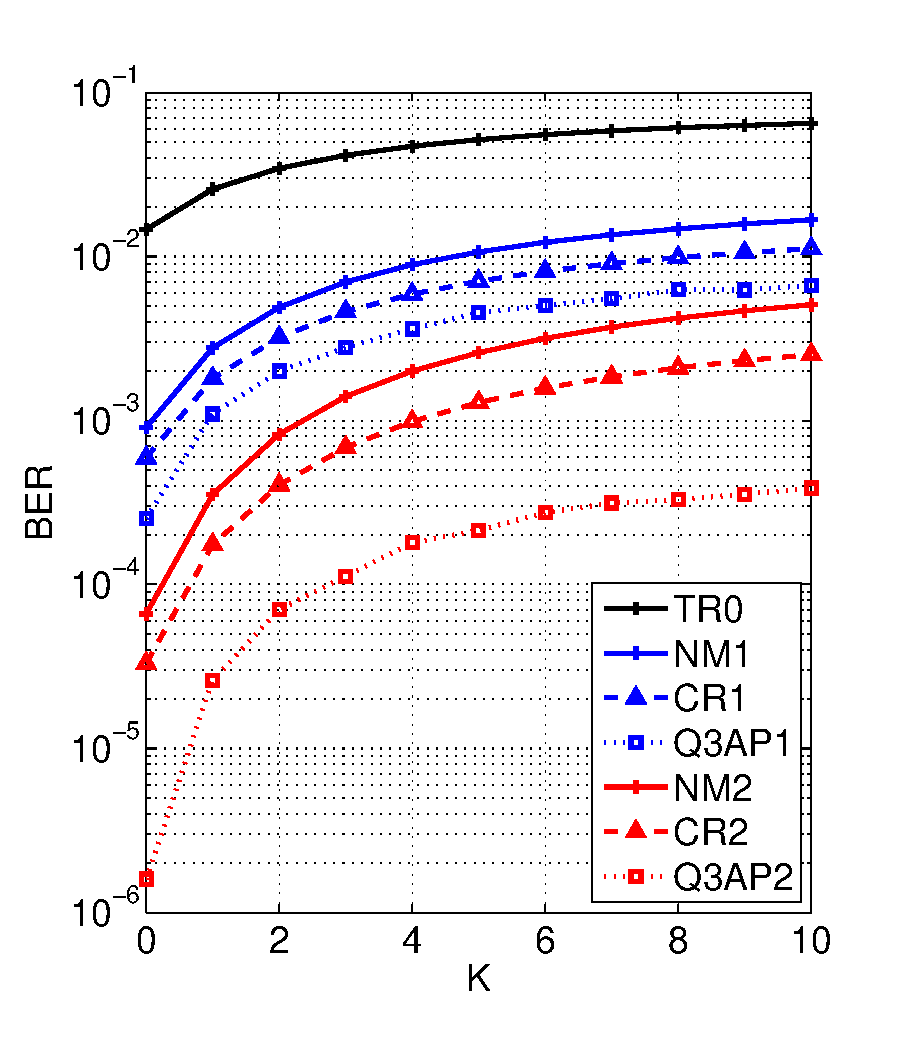
\includegraphics[width=4.5cm]{./figs/BER_K_MonteCarlo_64QAM_12.eps}}
    \centerline{(a) $m=1,2$}\medskip
  \end{minipage}
  \hfill
  \begin{minipage}[b]{0.48\linewidth}
    \centering
    \centerline{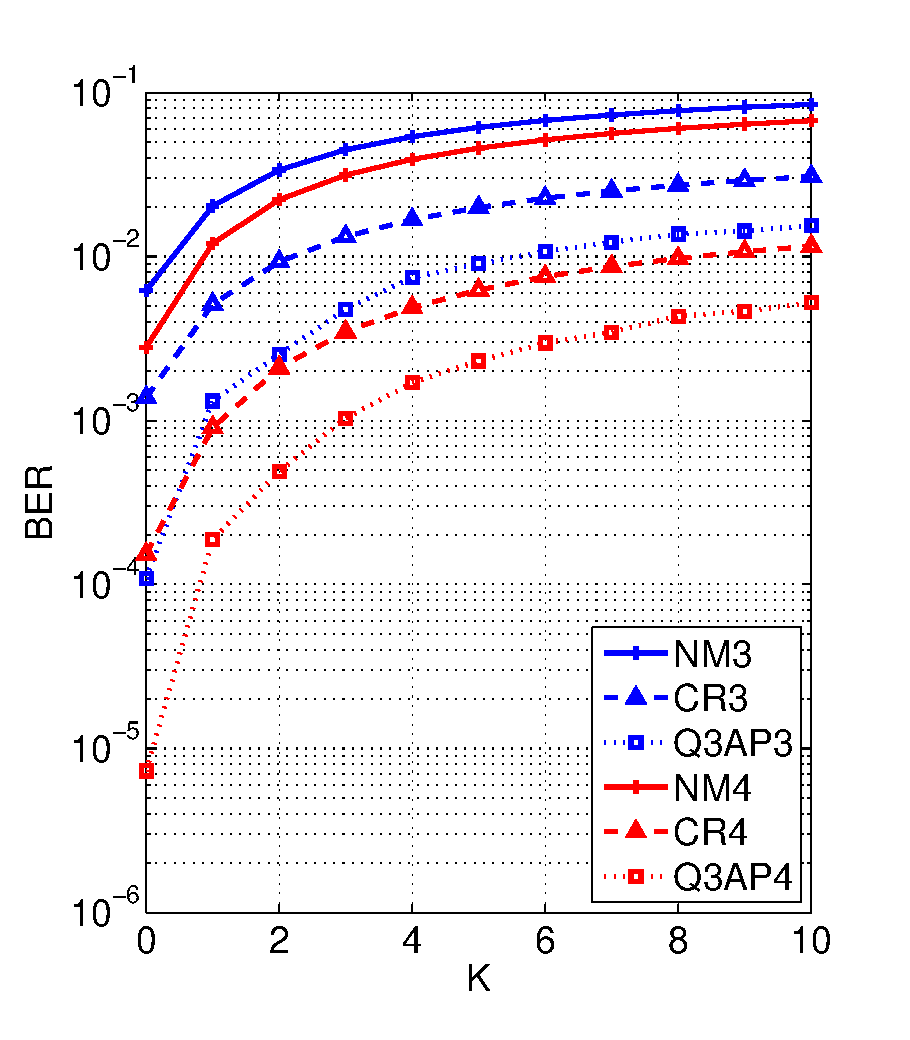
\includegraphics[width=4.5cm]{./figs/BER_K_MonteCarlo_64QAM_34.eps}}
    \centerline{(b) $m=3,4$}\medskip
  \end{minipage}
  \vspace{-10pt}
  \caption{Monte-Carlo simulation results of uncoded BER.}
  \label{fig:uncoded_K_mc}
\end{figure}

As another practical performance measurement, the coded BER performances of
the three MoDiv schemes are compared in a LDPC-coded system. A
LDPC code of length $L=2400$ and code rate $r=3/4$ is used. To demonstrate the
robustness of our Q3AP-based MoDiv scheme against design parameter mismatch, we
optimize the remapping only for $\sigma^2 = 5$dB and test the coded BER for a
wide range of $\sigma^2$. As shown in Fig.~\ref{fig:coded}, despite of the
mismatch in the design parameter $\sigma^2$, our Q3AP-based MoDiv is still able
to outmatches the other two MoDiv schemes, especially in the more likely
cases of a smaller number of retransmissions. 
Specifically, the waterfall curve of coded BER for  Q3AP1
almost overlaps with that of NM2, and Q3AP2 outperforms the other 2 schemes by
around 1.7dB and 4dB, respectively. The average HARQ
throughput defined in~\cite{panasonic2001enhanced} for the same LDPC coded
system is also shown in Fig.~\ref{fig:coded_throughput}, which further verifies
the performance gain of the Q3AP-based MoDiv design approach.
\begin{figure}[!t]
  \centering
  \begin{minipage}[b]{1\columnwidth}
    \centering
    \centerline{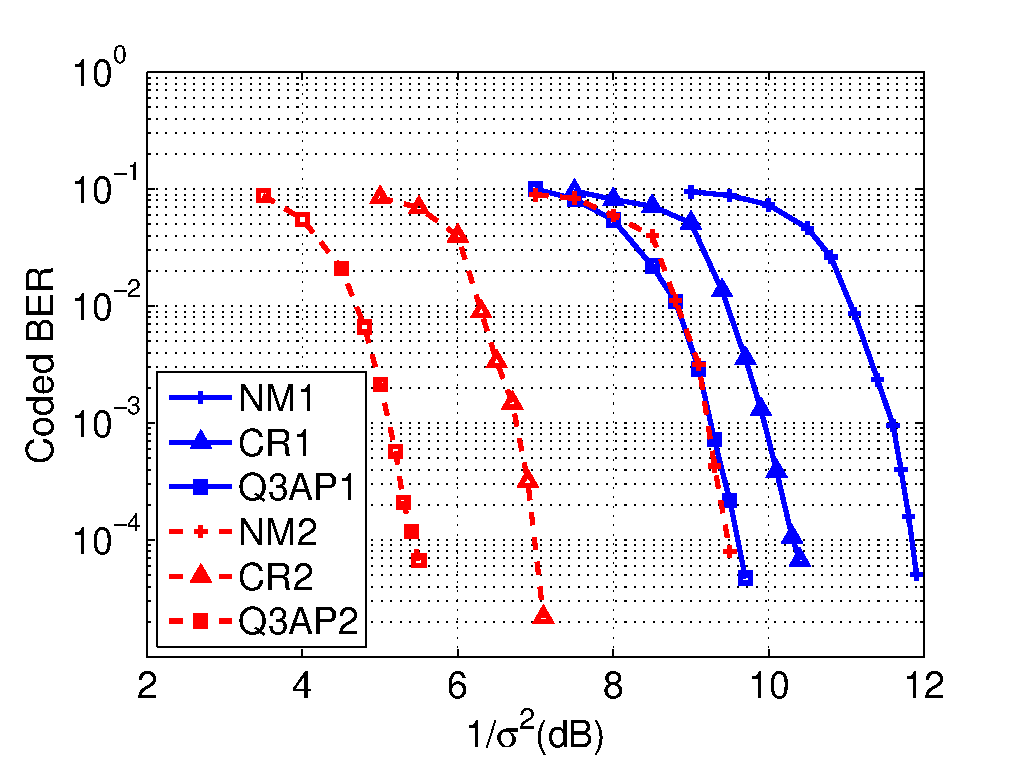
\includegraphics[width=6.5cm]{./figs/waterfall_64QAM_12.eps}}
    %\centerline{(a) $m=1,2$}\medskip
  \end{minipage}
  \hfill
  \begin{minipage}[b]{1\columnwidth}
    \centering
    \centerline{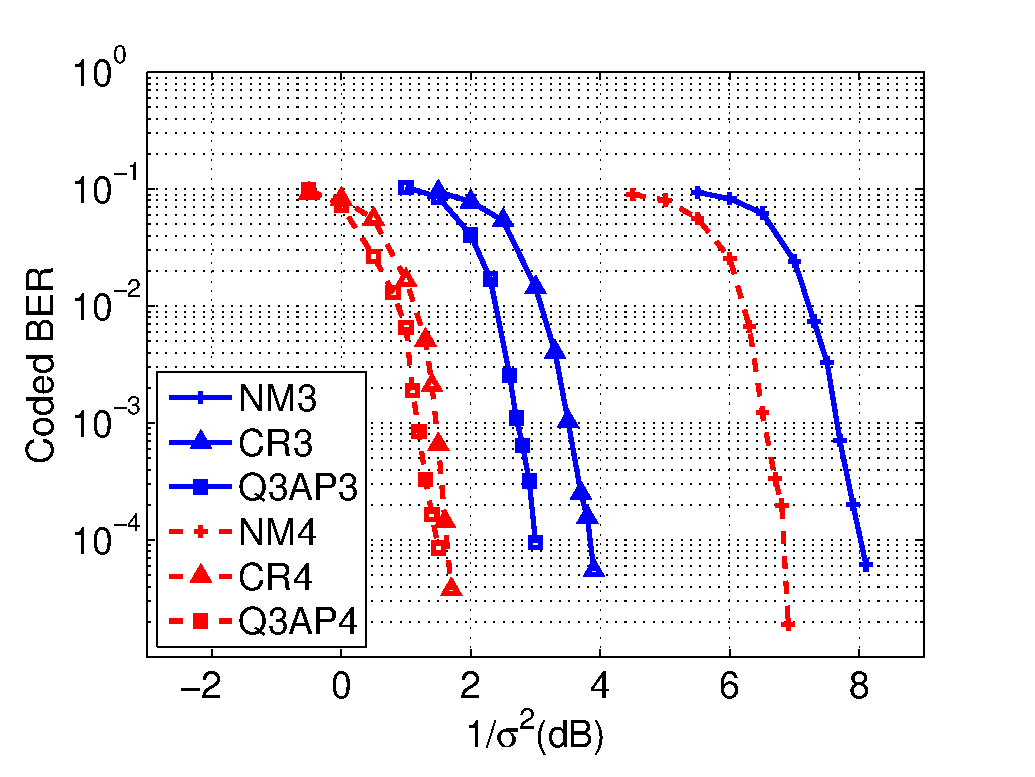
\includegraphics[width=6.5cm]{./figs/waterfall_64QAM_34.eps}}
    %\centerline{(b) $m=3,4$}\medskip
  \end{minipage}
  \vspace{-10pt}
  \caption{Coded BER. $m=1, 2$ (top) and $m=3,4$ (bottom).}
  \label{fig:coded}
\end{figure}
\begin{figure}[!t]
  \centering
  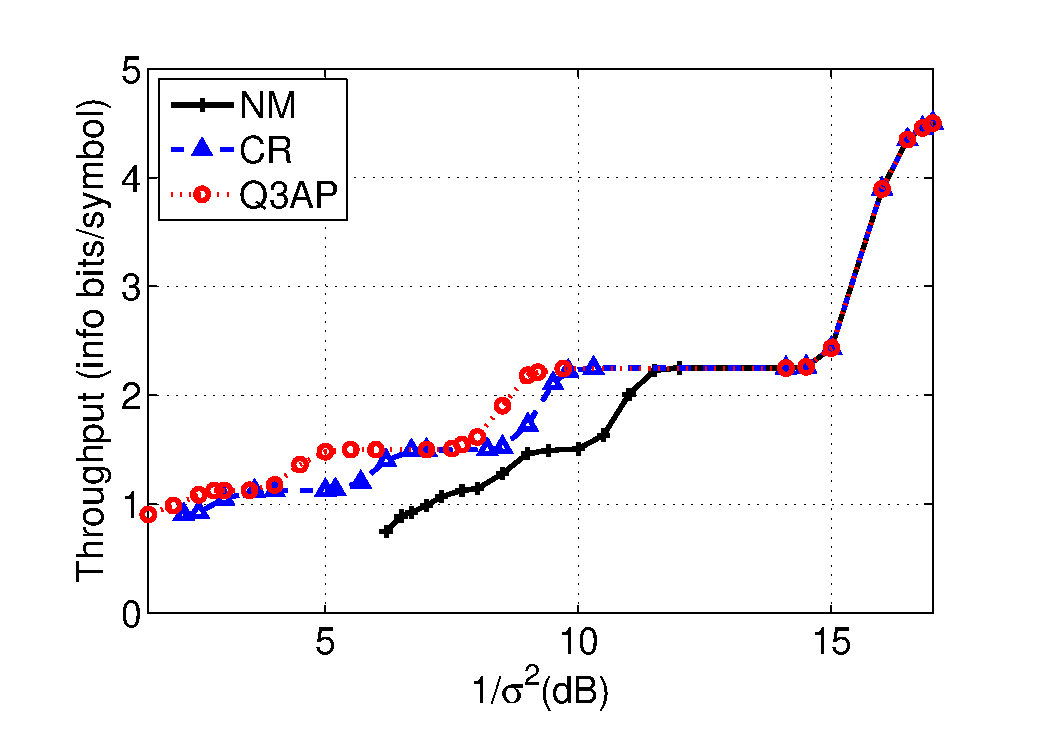
\includegraphics[width=0.75\columnwidth]{./figs/throughput.eps}
  \vspace{-10pt}
  \caption{Average throughput.}
  \label{fig:coded_throughput}
\end{figure}

\section{Conclusion}
\label{sec:conclusion}
In this work, we investigated the modulation diversity (MoDiv) design problem
for HARQ in a CoMP-MIMO system. Aiming to minimize the bit error rate (BER)
upper bound, we formulated the MoDiv design into a quadratic three-dimensional
assignment problem (Q3AP), and presented an efficient modified iterative local
search (ILS) solution. Our numerical tests demonstrate the performance advantage
and robustness of our MoDiv design over simply repeated use of Gray mapping
and an existing heuristic scheme.
% An example of a floating figure using the graphicx package.
% Note that \label must occur AFTER (or within) \caption.
% For figures, \caption should occur after the \includegraphics.
% Note that IEEEtran v1.7 and later has special internal code that
% is designed to preserve the operation of \label within \caption
% even when the captionsoff option is in effect. However, because
% of issues like this, it may be the safest practice to put all your
% \label just after \caption rather than within \caption{}.
%
% Reminder: the "draftcls" or "draftclsnofoot", not "draft", class
% option should be used if it is desired that the figures are to be
% displayed while in draft mode.
%
%\begin{figure}[!t]
%\centering
%\includegraphics[width=2.5in]{myfigure}
% where an .eps filename suffix will be assumed under latex, 
% and a .pdf suffix will be assumed for pdflatex; or what has been declared
% via \DeclareGraphicsExtensions.
%\caption{Simulation results for the network.}
%\label{fig_sim}
%\end{figure}

% Note that IEEE typically puts floats only at the top, even when this
% results in a large percentage of a column being occupied by floats.


% An example of a double column floating figure using two subfigures.
% (The subfig.sty package must be loaded for this to work.)
% The subfigure \label commands are set within each subfloat command,
% and the \label for the overall figure must come after \caption.
% \hfil is used as a separator to get equal spacing.
% Watch out that the combined width of all the subfigures on a 
% line do not exceed the text width or a line break will occur.
%
%\begin{figure*}[!t]
%\centering
%\subfloat[Case I]{\includegraphics[width=2.5in]{box}%
%\label{fig_first_case}}
%\hfil
%\subfloat[Case II]{\includegraphics[width=2.5in]{box}%
%\label{fig_second_case}}
%\caption{Simulation results for the network.}
%\label{fig_sim}
%\end{figure*}
%
% Note that often IEEE papers with subfigures do not employ subfigure
% captions (using the optional argument to \subfloat[]), but instead will
% reference/describe all of them (a), (b), etc., within the main caption.
% Be aware that for subfig.sty to generate the (a), (b), etc., subfigure
% labels, the optional argument to \subfloat must be present. If a
% subcaption is not desired, just leave its contents blank,
% e.g., \subfloat[].


% An example of a floating table. Note that, for IEEE style tables, the
% \caption command should come BEFORE the table and, given that table
% captions serve much like titles, are usually capitalized except for words
% such as a, an, and, as, at, but, by, for, in, nor, of, on, or, the, to
% and up, which are usually not capitalized unless they are the first or
% last word of the caption. Table text will default to \footnotesize as
% IEEE normally uses this smaller font for tables.
% The \label must come after \caption as always.
%
%\begin{table}[!t]
%% increase table row spacing, adjust to taste
%\renewcommand{\arraystretch}{1.3}
% if using array.sty, it might be a good idea to tweak the value of
% \extrarowheight as needed to properly center the text within the cells
%\caption{An Example of a Table}
%\label{table_example}
%\centering
%% Some packages, such as MDW tools, offer better commands for making tables
%% than the plain LaTeX2e tabular which is used here.
%\begin{tabular}{|c||c|}
%\hline
%One & Two\\
%\hline
%Three & Four\\
%\hline
%\end{tabular}
%\end{table}


% Note that the IEEE does not put floats in the very first column
% - or typically anywhere on the first page for that matter. Also,
% in-text middle ("here") positioning is typically not used, but it
% is allowed and encouraged for Computer Society conferences (but
% not Computer Society journals). Most IEEE journals/conferences use
% top floats exclusively. 
% Note that, LaTeX2e, unlike IEEE journals/conferences, places
% footnotes above bottom floats. This can be corrected via the
% \fnbelowfloat command of the stfloats package.



% if have a single appendix:
%\appendix[]

% or
%\appendix  % for no appendix heading
% do not use \section anymore after \appendix, only \section*
% is possibly needed

% use appendices with more than one appendix
% then use \section to start each appendix
% you must declare a \section before using any
% \subsection or using \label (\appendices by itself
% starts a section numbered zero.)
%




%Appendix one text goes here.

% you can choose not to have a title for an appendix
% if you want by leaving the argument blank
%\section{}
%Appendix two text goes here.


% use section* for acknowledgment
%\section*{Acknowledgment}


%The authors would like to thank...


% Can use something like this to put references on a page
% by themselves when using endfloat and the captionsoff option.
\ifCLASSOPTIONcaptionsoff
  \newpage
\fi



% trigger a \newpage just before the given reference
% number - used to balance the columns on the last page
% adjust value as needed - may need to be readjusted if
% the document is modified later
%\IEEEtriggeratref{8}
% The "triggered" command can be changed if desired:
%\IEEEtriggercmd{\enlargethispage{-5in}}

% references section

% can use a bibliography generated by BibTeX as a .bbl file
% BibTeX documentation can be easily obtained at:
% http://www.ctan.org/tex-archive/biblio/bibtex/contrib/doc/
% The IEEEtran BibTeX style support page is at:
% http://www.michaelshell.org/tex/ieeetran/bibtex/
\bibliographystyle{IEEEtran}
% argument is your BibTeX string definitions and bibliography database(s)
\bibliography{IEEEabrv,./refs.bib}

%
% <OR> manually copy in the resultant .bbl file
% set second argument of \begin to the number of references
% (used to reserve space for the reference number labels box)
%\begin{thebibliography}{1}

%\bibitem{IEEEhowto:kopka}
%H.~Kopka and P.~W. Daly, \emph{A Guide to \LaTeX}, 3rd~ed.\hskip 1em plus
%  0.5em minus 0.4em\relax Harlow, England: Addison-Wesley, 1999.

%\end{thebibliography}

% biography section
% 
% If you have an EPS/PDF photo (graphicx package needed) extra braces are
% needed around the contents of the optional argument to biography to prevent
% the LaTeX parser from getting confused when it sees the complicated
% \includegraphics command within an optional argument. (You could create
% your own custom macro containing the \includegraphics command to make things
% simpler here.)
%\begin{IEEEbiography}[{\includegraphics[width=1in,height=1.25in,clip,keepaspectratio]{mshell}}]{Michael Shell}
% or if you just want to reserve a space for a photo:

%\begin{IEEEbiography}{Michael Shell}
%Biography text here.
%\end{IEEEbiography}

% if you will not have a photo at all:
%\begin{IEEEbiographynophoto}{John Doe}
%Biography text here.
%\end{IEEEbiographynophoto}

% insert where needed to balance the two columns on the last page with
% biographies
%\newpage

%\begin{IEEEbiographynophoto}{Jane Doe}
%Biography text here.
%\end{IEEEbiographynophoto}

% You can push biographies down or up by placing
% a \vfill before or after them. The appropriate
% use of \vfill depends on what kind of text is
% on the last page and whether or not the columns
% are being equalized.

%\vfill

% Can be used to pull up biographies so that the bottom of the last one
% is flush with the other column.
%\enlargethispage{-5in}



% that's all folks
\end{document}


